%!TEX program = xelatex
\documentclass[algorithmlist,figurelist,tablelist,nomlist,masters]{seuthesix}
\usepackage{style}

\begin{document}
\categorynumber{000} % 分类采用《中国图书资料分类法》
\UDC{000}            %《国际十进分类法UDC》的类号
\secretlevel{公开}   % 学位论文密级分为"公开"、"内部"、"秘密"和"机密"四种
\studentid{140926}   % 学号要完整,前面的零不能省略
\title{大跨越输电塔结构在龙卷风作用下的响应分析}{}{Dynamic Response Analysis of Long Span Transmission Tower Structure Under Tornado Wind Loading}{}
\author{王勇}{Wang Yong}
\advisor{吕令毅}{教授}{Ling-yi Lv}{Prof.}
\degreetype{工学硕士}{Master of Engineering} % 详细学位名称
\major{土木工程}
\submajor{结构工程}
\defenddate{\today}
\authorizedate{\today}
\committeechair{}
\reviewer{}{}
\department{东南大学土木工程学院}{School of Civil Engineering}
%\seuthesisthanks{}

\makebigcover
\makecover

\begin{abstract}{}
\end{abstract}

\begin{englishabstract}{}
\end{englishabstract}

\tableofcontents

\mainmatter

\chapter{龙卷风风场及其数值模拟}

\section{龙卷风的特性及描述}
无论是模拟龙卷风,还是评估龙卷风对结构的影响,都需要对龙卷风的风场特性进行研究。
人们采用龙卷风的强度级数来衡量龙卷风造成的破坏的程度。
但由于龙卷风风场的复杂性,实际工程的抗龙卷风设计中,一般对其进行简化。
目前工程界主要通过给定龙卷风的特征参数以及通过Rankine涡模型中给定的龙卷风切向速度和压强等详细流场信息,来确定龙卷风对结构的影响。

\subsection{龙卷风的强度等级}
1970年,美国芝加哥大学的藤田(T. Theodore Fujita)教授提出将龙卷风按最大风速划分为7个等级,这种等级划分方法即为藤田级数。
但要直接测量龙卷风的最大风速并不容易,一般是根据龙卷风带来的破坏程度来估计龙卷风的最大风速,进而确定它的强度等级。

2007年2月1日起,美国气象部门采用改进的藤田级数(The Enhanced F-scale\cite{marshall2004enhanced})。
改进的藤田级数见表\ref{tab:EF_scale},分为EF0到EF5级。
它考虑了建筑物的坚固程度,对物体进行分类,共包括23种房屋以及5种非房屋类,如树木、桅杆等。
通过对给定各类物体的破坏描述,来估计龙卷风的最大风速,确定龙卷风的强度等级。
因此,改进的藤田级数能更准确地评估龙卷风的强度\cite{doswell2009implementation}。
\begin{table}[!htb]
\caption{龙卷风强度级数的划分}
\label{tab:EF_scale}
\centering
\begin{tabular*}{\textwidth}{c @{\extracolsep{\fill}} c p{11cm}}
    \toprule
    等级 & 风速(\SI{}{m/s}) & 破坏程度 \\ \midrule
    EF0 & $29.2-38.1$ & 轻度破坏:烟囱被损坏;刮断树枝;浅根系树木倾斜;毁坏商店招牌 \\
    EF1 & $38.3-49.4$ & 中度破坏:掀起屋顶的砖瓦;掀翻移动住房;行动汽车被刮离路面 \\
    EF2 & $49.7-60.6$ & 较严重破坏:刮走屋顶;摧毁活动住房;掀翻火车车厢;连根拔起大树;空中轻物乱飞;汽车被卷起 \\
    EF3 & $60.8-73.9$ & 严重破坏:坚固房屋屋顶和墙壁被刮走;掀翻火车;森林中大多数树木被连根拔起;重型汽车被卷离地然后被抛起 \\
    EF4 & $74.2-89.4$ & 毁灭性破坏:坚固房屋被整体刮倒;基础不牢的建筑物被刮跑;汽车被抛向空中,空中比较大的物件横飞 \\
    EF5 & $>89.4$ & 极度破坏:坚固房屋框架被刮走;汽车大小的物件在空中横飞超过100米;飘飞碎片挂树梢;出现很罕见的现象 \\
    \bottomrule
\end{tabular*}
\end{table}


\subsection{龙卷风的特征参数}
工程计算采用的龙卷风风场模型,具有如下参数:
(1)最大旋转风速$V_{\mathrm{R}}$;
(2)龙卷风涡的平移速度$V_{\mathrm{T}}$;
(3)最大旋转风速的半径$R$;
(4)气压降$\Delta P$;
(5)气压降速率$\mathrm{d} P/ \mathrm{d} t$。

我国《三十万千瓦压水堆核电厂安全重要土建结构抗龙卷风设计规定》中根据我国国情给出的两组龙卷风设计参数,如表\ref{tab:design_tornado}所示。除龙卷风发生概率低于$10^{-7}$的地区以外,根据厂址所在地区龙卷风资料的调研结果,从安全角度出发,选用一组合适的设计参数作为设计基准龙卷风\cite{EJ420}。
\begin{table}[!htbp]
\caption{设计基准龙卷风特性}
\label{tab:design_tornado}
\centering
\begin{tabular*}{\textwidth}{c @{\extracolsep{\fill}} c c c c c c}
    \toprule
    组 & 最大风速 & 旋转风速 & 平移风速 & 最大旋转半径 & 压力降 & 降压时间 \\
    别 & $V (\SI{}{m/s})$ & $V_{\mathrm{R}}  (\SI{}{m/s})$ & $V_{\mathrm{T}}  (\SI{}{m/s})$ & $R (\SI{}{m})$ & $\Delta P (\SI{}{Pa})$ & $t (\SI{}{s})$ \\ \midrule
    A & 107.3 & 84.9 & 22.4 & 45.7 & 8620 & 2.5 \\
    B & 134.1 & 107.3 & 28.8 & 45.7 & 13500 & 1.875 \\ \bottomrule
\end{tabular*}
\end{table}


\subsection{龙卷风的Rankine涡模型}
为了描述龙卷风风场的相关详细信息,工程界采用较多的是由Depperman\cite{Depperman1947}于1947年提出的Rankine涡模型。
Rankine涡模型是满足Navier-Stokes方程的最简单的模型,仅由切向速度控制。
它不考虑径向速度,并假定风速和压强不随高度变化,这在实际情况中是并不存在的。
但研究者最关心的也正是龙卷风的切向速度,因为相比于切向速度,龙卷风的径向速度和竖向速度较小。
其切向速度与离漩涡中心径向位置的关系曲线见图\ref{fig:Rankine}所示:强制涡区域内($r\leq R$)切向速度与半径成正比,而在自由涡区域内($r > R$)成反比。Rankine涡的切向速度表达式为\cite{Commission2007}:
\begin{equation}
\label{eqn:Rankine}
\begin{split}
    V_r &= \frac{r}{R} V_R,  \,\,\, r \leq R \\
    V_r &= \frac{R}{r} V_R,  \,\,\, r > R
\end{split}
\end{equation}
式中:$V_r$是距涡中心为$r$处的切向风速,$V_{\mathrm{R}}$为Rankine涡中的最大切向风速,$R$为最大切向风速对应的旋转半径。
\begin{figure}[!htbp]
\centering
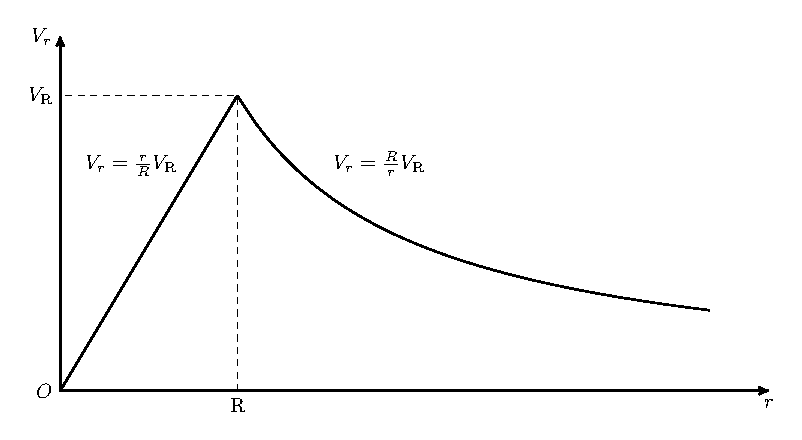
\includegraphics{tornado-simulation/fig/Rankine.pdf}
\caption{Rankine涡模型中切向速度沿涡半径的变化曲线图}
\label{fig:Rankine}
\end{figure}



\section{龙卷风的数值模拟}
实际情况中龙卷风的风场结构十分复杂,不仅有着单涡和多涡等多种形式,还具有一定的平移速度。
出于简化影响因素的考虑,本文仅模拟单涡形式的龙卷风,且不考虑龙卷风的平移运动,忽略地面粗糙度的影响。
采用计算流体力学软件FLUENT模拟缩尺龙卷风数值模型。


\subsection{风场几何区域}
为了与Baker\cite{baker1981boundary}的实验进行对比以验证数值风场的正确性,
将风场几何区域设置为与其实验装置尺寸类似的圆柱体,
具体尺寸及边界设置见图\ref{fig:tornado-domain}。
其中$X$轴对应龙卷风风场的径向,$Z$轴对应龙卷风风场的竖向。
\begin{figure}[!htbp]
  \centering
  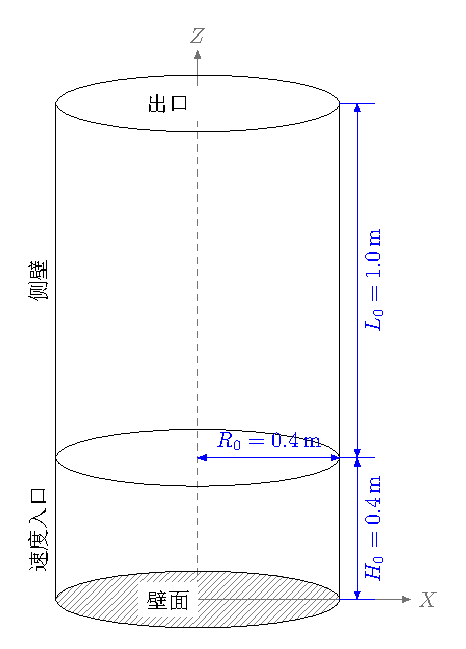
\includegraphics[width=0.6\textwidth]{tornado-simulation/fig/domain.pdf}
  \caption{龙卷风数值模型的几何区域}\label{fig:tornado-domain}
\end{figure}


\subsection{网格划分}
采用适应性良好的六面体结构化网格进行计算流域的划分。
由于工程实际主要关注近地面附近龙卷风对结构的作用,
故对近地面流域处的网格进行了细分。
进行初步的网格收敛性研究后,最终采用的结构化网格的数量为 \SI{3E5}{}。


\subsection{湍流模型}
龙卷风风场是旋流流场,根据Launder\cite{launder1989second}的研究,采用雷诺应力方程模型 (RSM)较为合适。
模型参数为:$C_{\mu}=0.09$; $C_{1\varepsilon}=1.44$; $C_{2\varepsilon}=1.92$; 
$C1-ps=1.8$; $C2-ps=0.6$; $C1'-ps=0.5$; $C2'-ps=0.3$。
湍流动能(TKE)普朗特数为 $1$; 湍动耗散率(TDR)普朗特数为 $1.3$。


\subsection{边界条件}
速度入口处径向和切向速度分布采用如下形式:
\begin{equation}\label{eqn:Vr}
  V_r(z) = V_0 \times (z/z_0)^{1/7}
\end{equation}
\begin{equation}\label{eqn:Vt}
  V_t(z) = 2 \times S \times V_r(z)
\end{equation}
式中,$V_r$为径向速度,$V_t$为切向速度,$V_0$为参考速度,$z_0$为参考高度,$S$为涡流比。

图\ref{fig:bc-inlet}为公式\eqref{eqn:Vr}和\eqref{eqn:Vt}所定义的风速分布与Baker\cite{baker1981boundary}试验的对比。
注意到试验风速分布与试验装置有关,而非实际的大气边界层风速分布。
公式\eqref{eqn:Vr}和\eqref{eqn:Vt}类似于大气边界层风速分布,并尽可能与Baker\cite{baker1981boundary}试验保持一致。
\begin{figure}[!htbp]
  \centering
  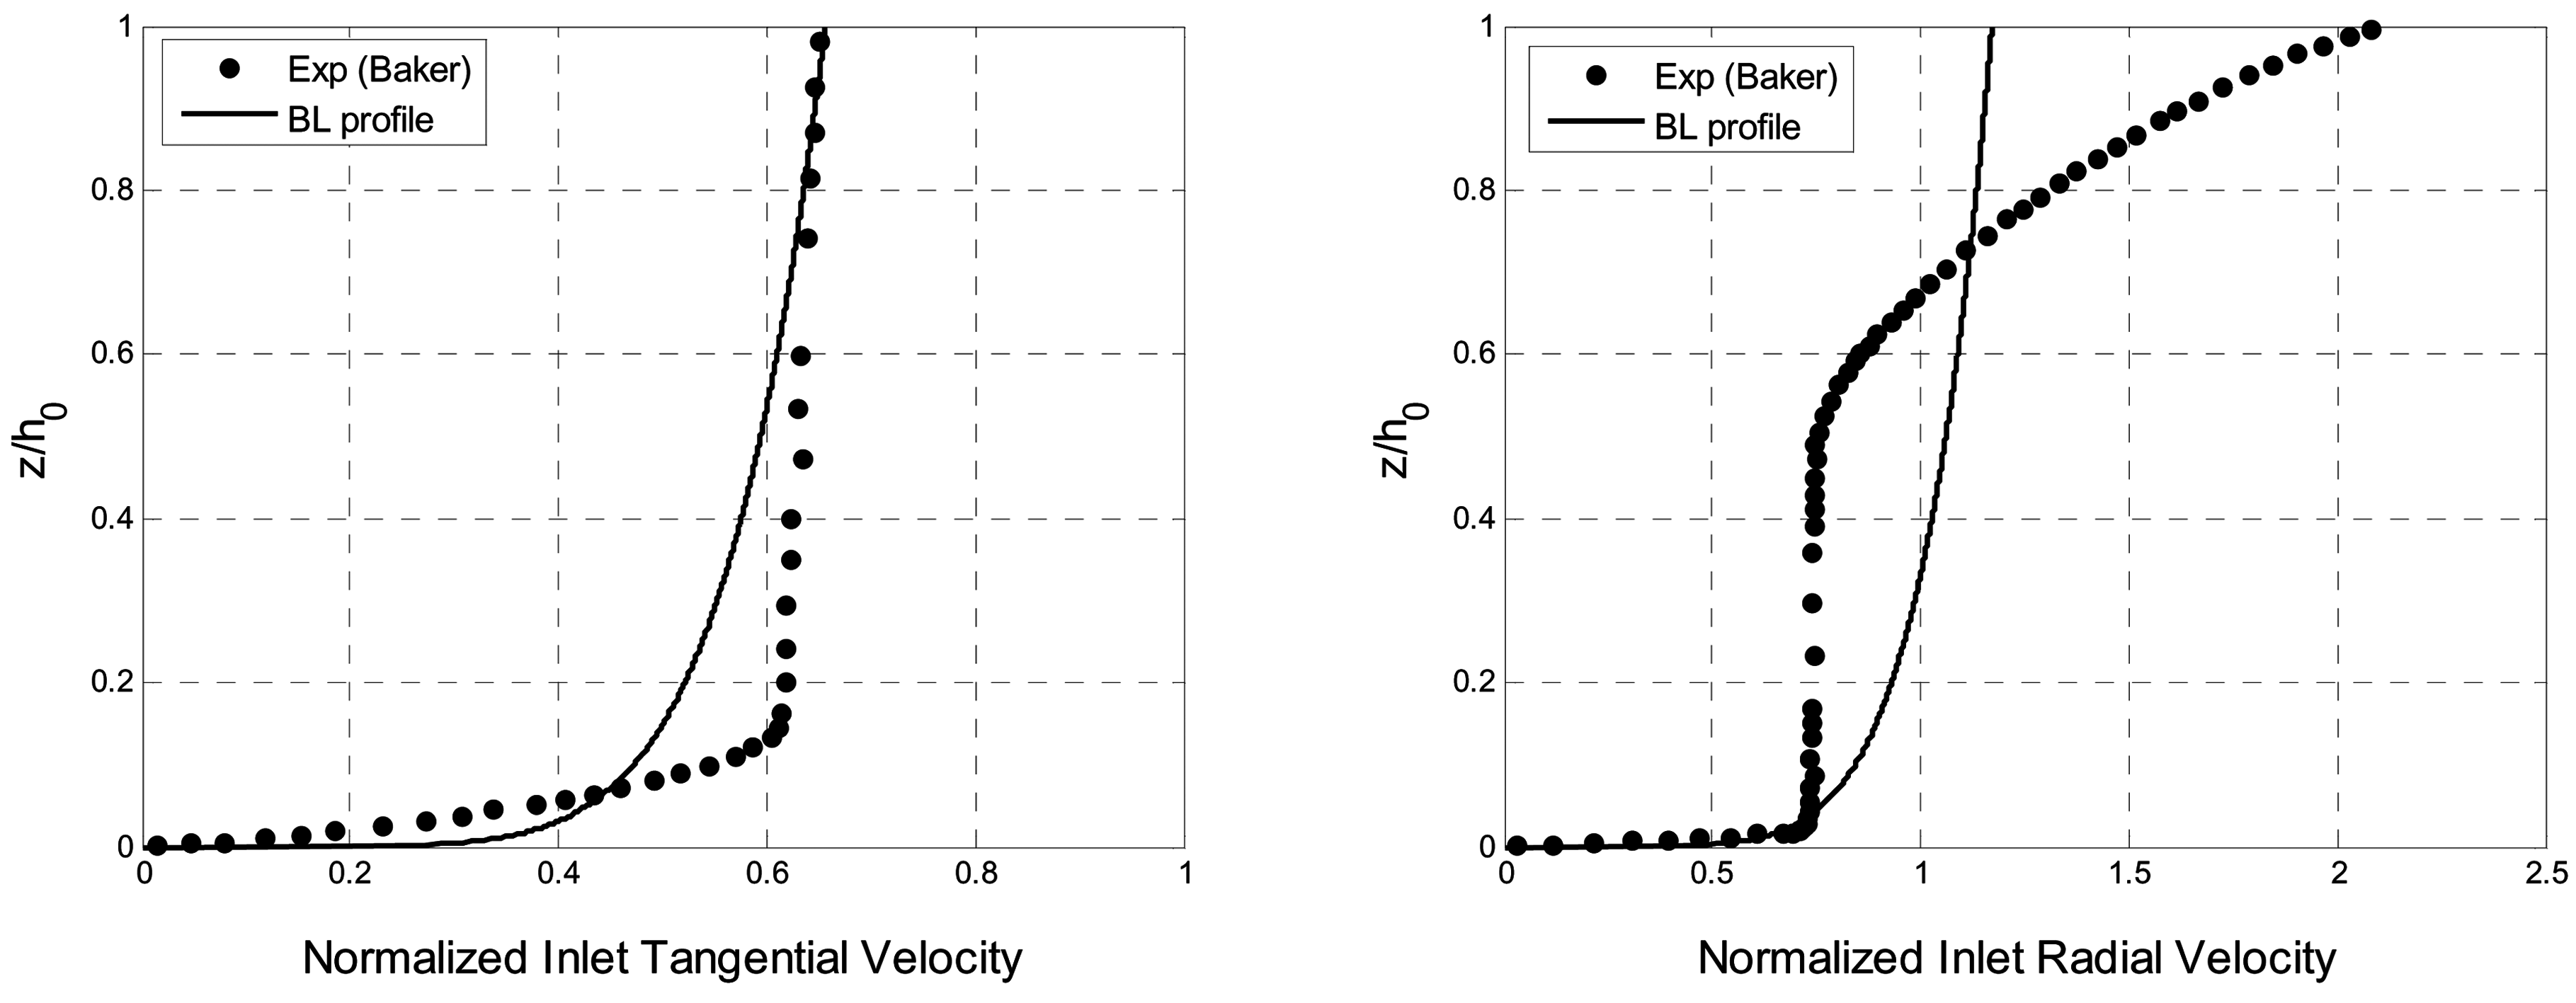
\includegraphics[width=\textwidth]{tornado-simulation/fig/bc_inlet.png}
  \caption{入口处规格化切向和径向速度与Baker\cite{baker1981boundary}试验的对比}
  \label{fig:bc-inlet}
\end{figure}

计算流域上边界采用出口边界条件。
此边界条件假设除压强外的所有物理量在边界的法向梯度为零\cite{fluent2015user}。

试验表明,沿壁面法线方向的不同距离,可以将近壁面区域分成三层区域。
最里层,又称粘性底层,流动区域很薄,粘性力在动量、热量及质量交换中都起主导作用;
最外层为对数率层,粘性力不起主要作用;
两层之间的区域为过渡层,粘性力作用与湍流作用相当。

为描述粘性底层和对数率层内的流动,现引入无量纲参数$u^{+}$和$y^{+}$:
\begin{equation}
  u^{+} = \frac{u}{u_{\tau}}
\end{equation}
\begin{equation}
  y^{+} = \frac{y u_{\tau}}{\nu} = \frac{y}{\nu} \sqrt{\frac{\tau_w}{\rho}}
\end{equation}
式中:$u$是流体的时均速度、$u_{\tau}=\sqrt{\tau_w/\rho}$为壁面摩擦速度、$\tau_w$为壁面处切应力、$\nu$为空气动粘度系数、$y$为壁面第一层节点到壁面的距离。

以$y^{+}$的对数为横坐标,以$u^{+}$为纵坐标,可将壁面区域内的三个区域表示为图\ref{fig:uplus}所示\cite{fluent2015theory}。
\begin{figure}[!htbp]
  \centering
  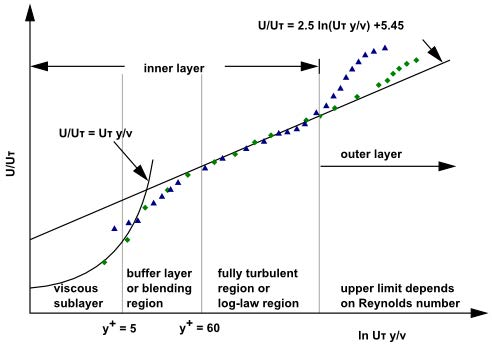
\includegraphics[width=0.6\textwidth]{tornado-simulation/fig/uplus.jpg}
  \caption{近壁面区域划分}\label{fig:uplus}
\end{figure}

通常有两种方法模拟近壁面区域:
一种采用“壁面方程”的半经验公式模拟受粘性力影响较大的区域,能够较好地修正湍流模型,解决壁面的存在对流场的影响;
另一种方法采用低$\mathrm{Re}$数的$k-\varepsilon$模型来求解粘性底层和过渡层,越靠近壁面,网格划分就越细,这种方法被称为“近壁面模型”法。
图\ref{fig:wall-treatment}为两种方法的对比\cite{fluent2015theory}。
\begin{figure}[!htbp]
  \centering
  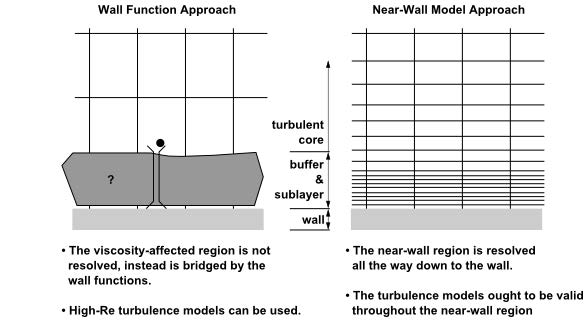
\includegraphics[width=0.8\textwidth]{tornado-simulation/fig/wall_treatment.jpg}
  \caption{近壁面区域处理方法}
  \label{fig:wall-treatment}
\end{figure}

本文壁面处采用强化壁面函数(Enhanced wall treatment\cite{fluent2015user}),需要对近壁面的网格进行细化。
边界层网格节点是否合适需要检查计算后的$y^{+}$值。
$y^{+}=u_{\tau} y/\nu$小于$1.5$能取得较好效果。


\subsection{控制方程及求解选项}
控制方程采用非定常雷诺平均纳维-斯托克斯方程(Unsteady Reynolds Averaged Navier-Stokes, RANS)。
时间离散采用一阶隐性格式,压强速度场的耦合采用压力修正的分离式算法,SIMPLEC算法。
动量、TKE、TDR和雷诺应力采用二阶迎风格式。


\thesisbib{seuthesix}

\end{document}
